\begin{center}
\fbox{\fbox{\parbox{6.5in}{\centering
\begin{flushleft}

\vspace{5mm}
\hspace{5mm}
\textbf{\underline{Võrdelised lõigud}}

\vspace{2mm}
\hspace{5mm}
Lõigud $a$ ja $b$ on \textbf{vastavalt võrdelised} lõikudega $y$ ja $x$, kui kehtib võrdus $\dfrac{a}{y}=\dfrac{b}{x}$.

\hspace{5mm}
Teisisõnu tähendab see seda, et lõikude suhted peavad olema võrdsed.

\hspace{5mm}
Esimese paari lõikude jagamisel peame saama tulemuseks täpselt samasuguse arvu, nagu teise paari\\ \hspace{5mm} lõikude jagamisel. Seda arvu nimetatakse \textbf{võrdeteguriks} ning tähistatakse tähega \textbf{$k$}.

\vspace{2mm}
\hspace{5mm}
Ehk:

\begin{equation}
\label{33_eq1}
\boxed{\dfrac{a}{y}=\dfrac{b}{x}=k}
\end{equation}

\vspace{2mm}
\hspace{5mm}
\textbf{Näiteks:} Oletame, et meil on pilt mis on veebilehe akna jaoks liiga pikk. Pildi kõrgus $a$ on $600$ pikslit,\\ \hspace{5mm} ning pildi laius $b$ on $318$ pikslit. Veebilehe akna kõrgus on aga hoopis $300$ pikslit. 

\vspace{2mm}
\hspace{5mm}
Vaatleme pildi kõrgust $a$ ja laiust $b$ kui üksikuid lõike.

\hspace{5mm}
On ilmselge, et pildi kõrgust tuleb teha poole väiksemaks (ehk jagada $2$-ga). Kuid kui me vähendaksime\\ \hspace{5mm} ainult pildi kõrgust, siis pildi laius jääks samaks ja pildil olev sisu oleks kokku surutud.

\vspace{2mm}
\hspace{5mm}
Kokkusurutud pilt meile aga ei sobi, kuna me sooviks ikkagi pildil olevat esialgset sisu säilitada.\\ \hspace{5mm} Proovime leida kui palju tuleb meil pildi laiust muuta.

\vspace{2mm}
\hspace{5mm}
Kui me jagame esialgse kõrguse $a$ uue kõrguse $y$-ga, siis leiame, et nende kahe kõrguse/lõigu jagatise\\ \hspace{5mm} tulemuseks saame arvu $2$.

\[ \dfrac{a}{y}=\dfrac{600}{300}=2 \]

\hspace{5mm}
See on ka meie võrdetegur, ehk $k=2$.

\hspace{5mm}
Järelikult, kui me nüüd peaksime võtma enda esialgse pildi laiuse $b$ ning jagama seda uue pildi\\ \hspace{5mm} laiusega $x$, ka siis peab meil jagatis võrduma $2$ - ga.  Ehk:

\[\dfrac{b}{x}=\dfrac{318}{x}=2 \hspace{3mm} \longrightarrow  \hspace{3mm}
x = \dfrac{318}{2}=159\]

\vspace{2mm}
\hspace{5mm}
\begin{tikzpicture}[scale=0.4]
\node[anchor=south west,inner sep=0] (image) at (0,0) {\includegraphics[scale=0.1]{metsik.jpg}};
  
  
\draw [<->] (-1,0)--(-1,11.25) node[left, pos=0.5]{$a=600$};
\draw[<->] (0,-1)--(6.25,-1) node[below, pos=0.5]{$b=318$};
\end{tikzpicture}
\hspace{10mm}
\begin{tikzpicture}[scale=0.4]
\node[anchor=south west,inner sep=0] (image) at (0,0) {\includegraphics[scale=0.1]{surutud.png}};
  
  
\draw [<->] (-1,0)--(-1,5.625) node[left, pos=0.5]{$y=300$};
\draw[<->] (0,-1)--(3.125,-1) node[below, pos=0.5]{$x=?$};
\end{tikzpicture}
\hspace{10mm}
\begin{tikzpicture}[scale=0.4]
\node[anchor=south west,inner sep=0] (image) at (0,0) {\includegraphics[scale=0.05]{metsik.jpg}};
  
  
\draw [<->] (-1,0)--(-1,5.625) node[left, pos=0.5]{$y=300$};
\draw[<->] (0,-1)--(3.125,-1) node[below, pos=0.5]{$x=159$};
\end{tikzpicture}

\vspace{2mm}
\hspace{5mm}
Vastus: Uue pildi laius $x$ on 159 pikslit ning kõrgus $y$ 300 pikslit.


\end{flushleft}
}}}
\end{center}




\begin{center}
\fbox{\fbox{\parbox{6.5in}{\centering
\begin{flushleft}

\vspace{2mm}
\hspace{5mm}
\textbf{\underline{Kiirteteoreem}}

\vspace{2mm}
\hspace{5mm}
Kui lõigata nurga haarasid paralleelsete sirgetega, siis ühel haaral tekkinud lõigud on võrdelised teise\\ \hspace{5mm} haara vastavate lõikudega.

\vspace{5mm}
\hspace{5mm}
\begin{tikzpicture}[scale=0.4]

\coordinate (O) at (0,0);
\coordinate (v) at (6,4);
\coordinate (u) at (7,0);

\draw (v)--(O)--(u);

\node[below] at (v){$v$};
\node[left] at (O){$O$};
\node[below] at (u){$u$};

\coordinate (s1) at (2,-2);
\coordinate (s2) at (2.5,5);
\coordinate (t1) at (4,-2);
\coordinate (t2) at (4.5,5);

\draw[dashed, thick] (s1)--(s2);
\draw[dashed, thick] (t1)--(t2);

\node[below left] at (s1){$s$};
\node[below left] at(t1){$t$};

\node[below left] at (2,0){$A$};
\node[below left] at (4,0){$B$};
\node[above left] at (2,1.5){$C$};
\node[above left] at (4,3){$D$};

\node [text width=12cm] at (23,2){Ehk kui $s \parallel t$ ning $s$ ja $t$ lõikavad haarasid $u$ ja $v$, siis $\dfrac{OA}{OC}=\dfrac{AB}{CD}=\dfrac{OB}{OD}$};
\end{tikzpicture}

\vspace{2mm}
\hspace{5mm}
Järeldus: Nurga haarade lõikamisel paralleelsete sirgetega tekivad võrdeliste külgedega kolmnurgad.

\[ \dfrac{OA}{OB}=\dfrac{OC}{OD}=\dfrac{AC}{BD} \]






\end{flushleft}
}}}
\end{center}
\vspace{0.5cm}

\textbf{Märkmed}\\
\vspace{2mm}
\begin{mdframed}[style=graphpaper]
\vspace{12cm}
\end{mdframed}